%%%%%%%%%%%%%%%%%%%%%%%%%%%%%%%%%%%%%%%%%%%%%%%%%%%%%%%%%%%%%%%%%%%%%%%%%%%%%%%%%%
\begin{frame}[fragile]\frametitle{}
\begin{center}
{\Large Data Evaluation}
\end{center}
\end{frame}



%%%%%%%%%%%%%%%%%%%%%%%%%%%%%%%%%%%%%%%%%%%%%%%%%%%%%%%%%%
\begin{frame}
\frametitle{Example}
A certain disease has an incidence rate of 5\%.  %If the false negative rate is 8\% and the false positive rate is 3\%, compute the probability that a person who tests positive actually has the disease.\\

\vspace{.1in}
Imagine 10,000 people who are tested.\\ 
\begin{center}
\begin{tabular}{|l|c|c|c|}
\hline
& Positive & Negative &Total\\
\hline
Have disease & &&\\
\hline
Do not have disease && &\\
\hline
Total &&&10,000\\
\hline
\end{tabular}
\end{center}
\end{frame}

%%%%%%%%%%%%%%%%%%%%%%%%%%%%%%%%%%%%%%%%%%%%%%%%%%%%%%%%%%
\begin{frame}
\frametitle{Example}
%A certain disease has an incidence rate of 5\%.  If the false negative rate is 8\% and the false positive rate is 3\%, compute the probability that a person who tests positive actually has the disease.\\

\vspace{.1in}
Of these 10,000, 500 will have the disease.\\ 
\begin{center}
\begin{tabular}{|l|c|c|c|}
\hline
& Positive & Negative &Total\\
\hline
Have disease & &&500\\
\hline
Do not have disease && &\\
\hline
Total &&&10,000\\
\hline
\end{tabular}
\end{center}
\end{frame}

%%%%%%%%%%%%%%%%%%%%%%%%%%%%%%%%%%%%%%%%%%%%%%%%%%%%%%%%%%
\begin{frame}
\frametitle{Example}
%A certain disease has an incidence rate of 5\%.  If the false negative rate is 8\% and the false positive rate is 3\%, compute the probability that a person who tests positive actually has the disease.\\

\vspace{.1in}
Of these 10,000, 9,500 will not.\\ 
\begin{center}
\begin{tabular}{|l|c|c|c|}
\hline
& Positive & Negative &Total\\
\hline
Have disease & &&500\\
\hline
Do not have disease && &9,500\\
\hline
Total &&&10,000\\
\hline
\end{tabular}
\end{center}
\end{frame}

%%%%%%%%%%%%%%%%%%%%%%%%%%%%%%%%%%%%%%%%%%%%%%%%%%%%%%%%%%
\begin{frame}
\frametitle{Please Note}
\begin{itemize}
\item  If the outcome from a prediction is positive and the actual value is also positive, then it is called a true positive (TP);
\item However if the actual value is n then it is said to be a false positive (FP). Conversely, a true negative (TN) has occurred when both the prediction outcome and the actual value are n, and false negative (FN) is when the prediction outcome is n while the actual value is p.
\end{itemize}
\end{frame}

%%%%%%%%%%%%%%%%%%%%%%%%%%%%%%%%%%%%%%%%%%%%%%%%%%%%%%%%%%
\begin{frame}
\frametitle{Please Note}
\begin{center}
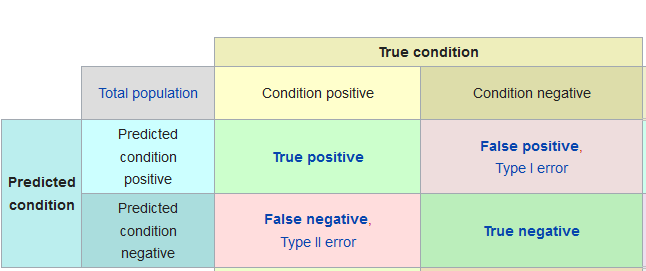
\includegraphics[width=\linewidth,keepaspectratio]{confmat}
\end{center}
\end{frame}


%%%%%%%%%%%%%%%%%%%%%%%%%%%%%%%%%%%%%%%%%%%%%%%%%%%%%%%%%%
\begin{frame}
\frametitle{Please Note}
\begin{center}
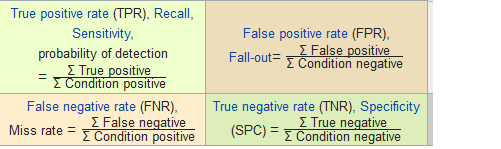
\includegraphics[width=\linewidth,keepaspectratio]{confrate}
\end{center}
\end{frame}

%%%%%%%%%%%%%%%%%%%%%%%%%%%%%%%%%%%%%%%%%%%%%%%%%%%%%%%%%%
\begin{frame}
\frametitle{Please Note}
\begin{center}
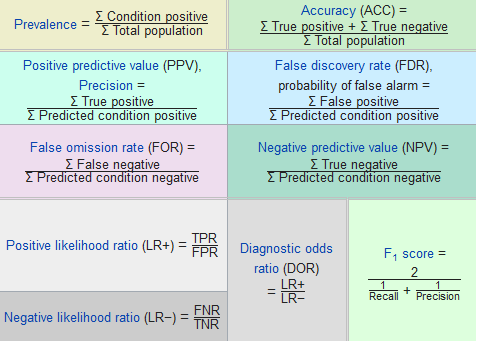
\includegraphics[width=\linewidth,keepaspectratio]{conff1}
\end{center}
\end{frame}
%%%%%%%%%%%%%%%%%%%%%%%%%%%%%%%%%%%%%%%%%%%%%%%%%%%%%%%%%%
\begin{frame}
\frametitle{Example}
%A certain disease has an incidence rate of 5\%.  
If the false negative rate is 8\% ie ``negative'' means test said negative but that is ``false'', means having a disease; 
% and the false positive rate is 3\%, compute the probability that a person who tests positive actually has the disease.\\

\vspace{.1in}
Of those with the disease, 8\% or 40 will test negative.\\ 
\begin{center}
\begin{tabular}{|l|c|c|c|}
\hline
& Positive & Negative &Total\\
\hline
Have disease & &40&500\\
\hline
Do not have disease && &9,500\\
\hline
Total &&&10,000\\
\hline
\end{tabular}
\end{center}
\end{frame}

%%%%%%%%%%%%%%%%%%%%%%%%%%%%%%%%%%%%%%%%%%%%%%%%%%%%%%%%%%
\begin{frame}
\frametitle{Example}
%A certain disease has an incidence rate of 5\%.  If the false negative rate is 8\% and the false positive rate is 3\%, compute the probability that a person who tests positive actually has the disease.\\

\vspace{.1in}
So remaining 460 who are having disease, will test positive.\\ 
\begin{center}
\begin{tabular}{|l|c|c|c|}
\hline
& Positive & Negative &Total\\
\hline
Have disease &460 &40&500\\
\hline
Do not have disease && &9,500\\
\hline
Total &&&10,000\\
\hline
\end{tabular}
\end{center}
\end{frame}

%%%%%%%%%%%%%%%%%%%%%%%%%%%%%%%%%%%%%%%%%%%%%%%%%%%%%%%%%%
\begin{frame}
\frametitle{Example}
%A certain disease has an incidence rate of 5\%.  If the false negative rate is 8\% and 
The false positive rate is 3\%, ie ``positive'' means the test predictive positive, but that is ``false'' means healthy or not having disease; 
%compute the probability that a person who tests positive actually has the disease.\\

\vspace{.1in}
Of the 9,500 who do not have the disease, 285, or 3\%, will test positive.\\ 
\begin{center}
\begin{tabular}{|l|c|c|c|}
\hline
& Positive & Negative &Total\\
\hline
Have disease &460 &40&500\\
\hline
Do not have disease &285& &9,500\\
\hline
Total &&&10,000\\
\hline
\end{tabular}
\end{center}
\end{frame}

%%%%%%%%%%%%%%%%%%%%%%%%%%%%%%%%%%%%%%%%%%%%%%%%%%%%%%%%%%
\begin{frame}
\frametitle{Example}
%A certain disease has an incidence rate of 5\%.  If the false negative rate is 8\% and the false positive rate is 3\%, compute the probability that a person who tests positive actually has the disease.\\

\vspace{.1in}
So ermaining 9,215 will test negative.\\ 
\begin{center}
\begin{tabular}{|l|c|c|c|}
\hline
& Positive & Negative &Total\\
\hline
Have disease &460 &40&500\\
\hline
Do not have disease &285&9,215 &9,500\\
\hline
Total &&&10,000\\
\hline
\end{tabular}
\end{center}
\end{frame}

%%%%%%%%%%%%%%%%%%%%%%%%%%%%%%%%%%%%%%%%%%%%%%%%%%%%%%%%%%
\begin{frame}
\frametitle{Example}
%A certain disease has an incidence rate of 5\%.  If the false negative rate is 8\% and the false positive rate is 3\%, compute the probability that a person who tests positive actually has the disease.\\

\vspace{.1in}
Fill in the totals.\\ 
\begin{center}
\begin{tabular}{|l|c|c|c|}
\hline
& Positive & Negative &Total\\
\hline
Have disease &460 &40&500\\
\hline
Do not have disease &285& 9,215&9,500\\
\hline
Total &745&9,255&10,000\\
\hline
\end{tabular}
\end{center}

So of the 745 total people who test positive, 460 will have the disease.  Thus 
\begin{equation*}
P(\hbox{disease}|\hbox{positive})=\frac{460}{745} \simeq 0.617,
\end{equation*}
\end{frame}


%%%%%%%%%%%%%%%%%%%%%%%%%%%%%%%%%%%%%%%%%%%%%%%%%%%%%%%%%%%
\begin{frame}[fragile]\frametitle{Errors}
\begin{itemize}
\item Type I- researcher rejects a null hypothesis when it is actually true.(FN)
\item Type II- researcher accepts a null hypothesis that is actually false.(FP)
\item Type I errors more serious, why?
\end{itemize}
\end{frame}


%%%%%%%%%%%%%%%%%%%%%%%%%%%%%%%%%%%%%%%%%%%%%%%%%%%%%%%%%%%
\begin{frame}[fragile]\frametitle{Errors}
\begin{center}
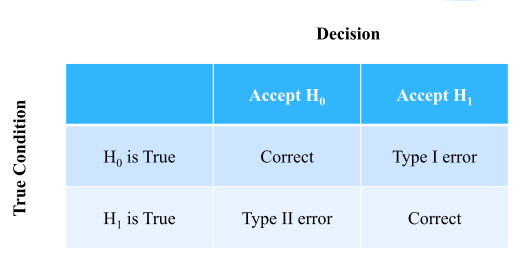
\includegraphics[width=\linewidth,keepaspectratio]{hoerrors}
\end{center}
\end{frame}

%
%\begin{frame}
%\frametitle{Joint distributions}
%
%Suppose we have two random variables that are measured together.
%Commonly this arises when two characteristics are measured for each
%unit in the sample.
%
%For example, suppose we have a sample of patients who were treated
%with one of two drugs, A and B.  The patient can experience a
%``complete response'' (CR), ``partial response'' (PR), or ``no
%response'' (NR).  The probabilities for all combinations of treatment
%type and response type might be as follows:
%
%\begin{center}
%\begin{tabular}{llll}
%   & CR & PR & NR \\\hline
%A  & 0.04 & 0.2 & 0.16\\
%B  & 0.18 & 0.06 & 0.36\\\hline
%\end{tabular}
%\end{center}
%
%This is called a {\bf joint distribution} (note that the probabilities
%sum to $1$).  We can express specific points in the distribution in
%the form ``$P(\cdot,\cdot) = \cdot$'' -- for example, $P(A, {\rm PR})
%= 0.2$.
%
%\end{frame}
%
%
%\begin{frame}
%\frametitle{Marginal distributions}
%
%By totaling within the rows and columns of the joint probability table
%we obtain the {\bf marginal distributions}:
%
%\begin{center}
%\begin{tabular}{llll|l}
%   & CR & PR & NR \\\hline
%A  & 0.04 & 0.20 & 0.16 & 0.4\\
%B  & 0.18 & 0.06 & 0.36 & 0.6\\\hline
%   & 0.22 & 0.26 & 0.52\\
%\end{tabular}
%\end{center}
%
%The marginal distribution of treatments is $P({\rm A})=0.4$, $P({\rm
%B})=0.6$; the marginal distribution of outcomes is $P({\rm CR})=0.22$,
%$P({\rm PR})=0.26$ and $P({\rm NR})=0.52$.
%
%\end{frame}
%
%
%\begin{frame}
%\frametitle{Conditional distributions}
%
%Now if we divide each row by its marginal probability, we get the
%row-wise {\bf conditional probabilities}:
%
%\begin{center}
%\begin{tabular}{llll}
%   & CR & PR & NR \\\hline
%A  & 0.1 & 0.5 & 0.4 \\
%B  & 0.3 & 0.1 & 0.6 \\\hline
%\end{tabular}
%\end{center}
%
%We can express these probabilities in the form ``$P(\cdot|\cdot) =
%\cdot$'' -- for example, $P({\rm PR}|{\rm B}) = 0.1$.
%
%Note that each row sums to 1, so each row is a separate probability
%distribution.
%
%If we denote the drug by ${\rm D}={\rm A},{\rm B}$ and the response by
%${\rm R}={\rm CR},{\rm PR},{\rm NR}$, then the overall conditional
%distribution is denoted $P({\rm R}|{\rm D})$.
%
%\end{frame}
%
%
%\begin{frame}
%\frametitle{Conditional distributions}
%
%If we divide each column by its marginal probability, we get the
%column-wise conditional probabilities:
%
%\begin{center}
%\begin{tabular}{llll}
%   & CR & PR & NR \\\hline
%A  & 0.18 & 0.77 & 0.31 \\
%B  & 0.82 & 0.23 & 0.69 \\\hline
%\end{tabular}
%\end{center}
%
%We can express these probabilities as $P({\rm B}|{\rm PR}) = 0.23$,
%for example.
%
%Note that each column sums to 1, so each column is a separate
%probability distribution.
%
%\end{frame}
%
%
%\begin{frame}
%\frametitle{Conditional expectation}
%
%Now suppose that one of the variables in our joint distribution is
%quantitative.  In this case, we are able to summarize the conditional
%distributions using the {\bf conditional expectation}.
%
%\textcolor{blue}{\bf Example:} Suppose we are evaluating new drugs A and
%B, and our interest is the maximum tolerable dose (MTD).  If the
%design of the study is such that the doses given are either 200, 400,
%or 600 mg/day, we might get the following joint probability
%distribution:
%
%\begin{center}
%\begin{tabular}{llll}
%   & \multicolumn{3}{c}{\rm MTD}\\
%   & 200 & 400 & 600 \\\hline
%A  & 0.04 & 0.20 & 0.16\\
%B  & 0.18 & 0.06 & 0.36\\\hline
%\end{tabular}
%\end{center}
%
%\end{frame}
%
%
%\begin{frame}
%\frametitle{Conditional expectation}
%
%The row-wise conditional distributions are:
%
%\begin{center}
%\begin{tabular}{llll}
%   & \multicolumn{3}{c}{\rm MTD}\\
%   & 200  & 400  & 600 \\\hline
%A  & 0.1 & 0.5 & 0.4 \\
%B  & 0.3 & 0.1 & 0.6 \\\hline
%\end{tabular}
%\end{center}
%
%Since each row of this table is a probability distribution, we can
%compute its expected value.  These are the conditional expectations.
%They tell us the expected MTD value for people who are treated with a
%particular drug.
%
%$$
%\begin{array}{ccccc}
%E({\rm MTD} | {\rm A}) &=& 0.1\cdot 200 + 0.5\cdot 400 + 0.4\cdot 600 &=& 460\\
%E({\rm MTD} | {\rm B}) &=& 0.3\cdot 200 + 0.1\cdot 400 + 0.6\cdot 600 &=& 460
%\end{array}
%$$
%
%Note that the conditional means are the same in this example, even
%though the conditional distributions differ.
%
%\end{frame}
%
%
%\begin{frame}
%\frametitle{Conditional expectation}
%
%Suppose now we have a different joint distribution table 
%
%\begin{center}
%\begin{tabular}{llll}
%   & \multicolumn{3}{c}{\rm MTD}\\
%   & 200  & 400  & 600 \\\hline
%A  & 0.24 & 0.12 & 0.04 \\
%B  & 0.06 & 0.30 & 0.24 \\\hline
%\end{tabular}
%\end{center}
%
%with row-wise conditional distributions:
%
%\begin{center}
%\begin{tabular}{llll}
%   & \multicolumn{3}{c}{\rm MTD}\\
%   & 200  & 400  & 600 \\\hline
%A  & 0.6 & 0.3 & 0.1 \\
%B  & 0.1 & 0.5 & 0.4 \\\hline
%\end{tabular}
%\end{center}
%
%In this case the conditional MTD expectations differ for the two
%drugs:
%
%$$
%\begin{array}{ccccc}
%E({\rm MTD} | {\rm A}) &=& 0.6\cdot 200 + 0.3\cdot 400 + 0.1\cdot 600 &=& 300\\
%E({\rm MTD} | {\rm B}) &=& 0.1\cdot 200 + 0.5\cdot 400 + 0.4\cdot 600 &=& 460
%\end{array}
%$$
%
%
%\end{frame}
%
%
%\begin{frame}
%\frametitle{Double expectation theorem}
%
%An important and useful fact called the {\bf double expectation
%theorem} relates conditional expectations and unconditional
%expectations.  The theorem states that for random variables $X$ and
%$Y$,
%
%$$
%EY = E_X E(Y|X).
%$$
%
%What this means is that we first calculate $E(Y|X)$, then average
%these values using the marginal distribution $P(X)$ as weights.  The
%result is $EY$.
%
%The notation $E_X$ stands for expectation, with the subscript $X$
%emphasizing that the expectation is taken with respect to the
%distribution of $X$.
%
%\end{frame}
%
%
%\begin{frame}
%\frametitle{Double expectation theorem}
%
%As an example, continuing from above we have $E({\rm MTD} | {\rm A}) =
%300$ and $E({\rm MTD} | {\rm B}) = 460$. Since $P({\rm A}) = 0.4$ and
%$P({\rm B}) = 0.6$, the double expectation theorem tells us that
%
%$$ E({\rm MTD}) = E({\rm MTD} | {\rm A})\cdot P({\rm A}) + E({\rm MTD}
%| {\rm B})\cdot P({\rm B}) = 300\cdot 0.4 + 460\cdot 0.6 = 396.
%$$
%
%The marginal distribution of MTD is $P({\rm MTD}=200) = 0.3$, $P({\rm
%MTD}=400) = 0.42$, and $P({\rm MTD}=600) = 0.28$.
%
%Calculating the marginal expected value $E{\rm MTD}$ directly yields
%
%$$
%E({\rm MTD}) = 0.3\cdot 200 + 0.42\cdot 400 + 0.28\cdot 600 = 396.
%$$
%
%Using the double expectation theorem here is the long way around, but
%we will see situations later where it is extremely useful.
%
%\end{frame}
%
%
%\begin{frame}
%\frametitle{Exercises}
%
%\begin{center}
%\begin{tabular}{cc|cc}
%  && \multicolumn{2}{c}{$Y$}\\
%  && 2   & 3   \\\hline
%\multirow{2}{*}{$X$} & 0 & 0.2 & 0.1 \\
%& 1 & 0.4 & 0.3 \\
%\end{tabular}
%\end{center}
%
%\begin{enumerate}
%
%\item Calculate the marginal distributions of $X$ and $Y$.
%
%\item Calculate $EX$ and $EY$.
%
%\item Calculate the conditional distribution of $X$ given $Y$ and the
%  conditional distribution of $Y$ given $X$.
%
%\item Use the double expectation theorem to calculate $EX$ from
%  $P(X|Y)$ and $P(Y)$, and to calculate $EY$ from $P(Y|X)$ and $P(X)$.
%
%\end{enumerate}
%
%\end{frame}
%
%
%\begin{frame}
%\frametitle{Conditional expectation of continuous values}
%
%If $X$ is continuous, the bivariate data $X,Y$ are usually displayed
%as a scatterplot rather than a table of counts.
%
%But we still have conditional expectations: $E(Y|X=x)$ is the
%population mean of $Y$ over all $X,Y$ pairs in which $X=x$.
%
%\end{frame}
%
%
%\begin{frame}
%\frametitle{Conditional expectation of continuous values}
%
%This scatterplot of $Y$ versus $X$ shows the population conditional
%mean function $E(Y|X)$ drawn in orange.
%
%\begin{center}
%\scalebox{0.6}{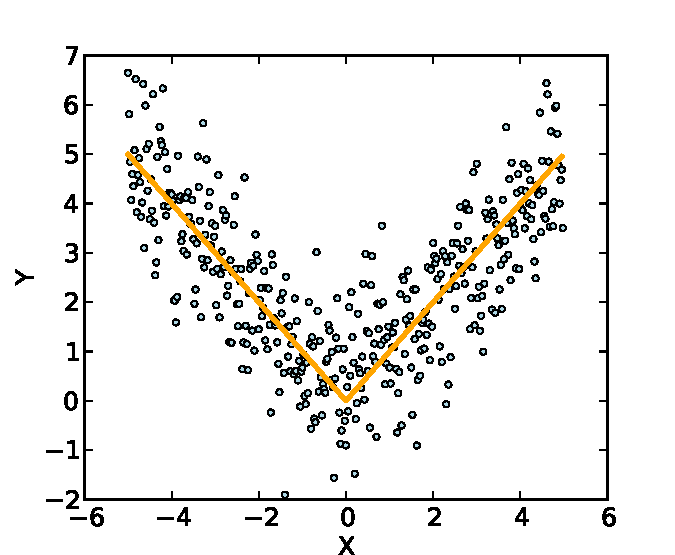
\includegraphics{011.pdf}}
%\end{center}
%
%\end{frame}
%
%
%\begin{frame}
%\frametitle{Conditional expectation of continuous values}
%
%Note that in each narrow vertical slice, the sample mean of the $Y$
%coordinates of the points in the slice is close to $E(Y|X)$:
%
%\begin{center}
%\scalebox{0.6}{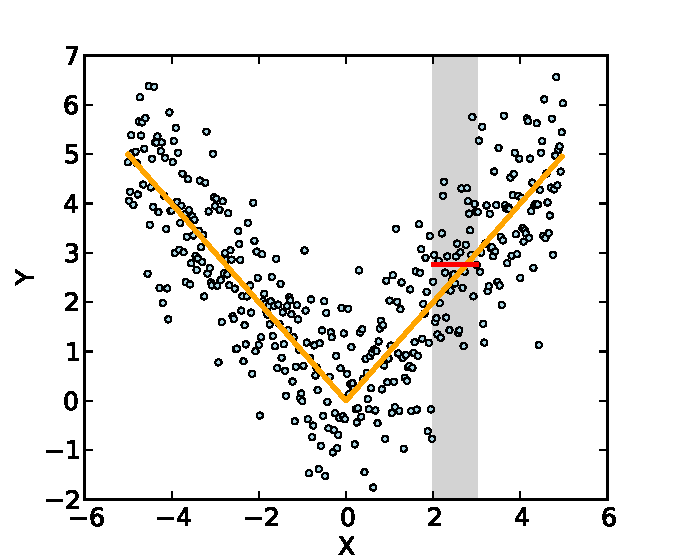
\includegraphics{012.pdf}}
%\end{center}
%
%\end{frame}
%
%
%\begin{frame}
%\frametitle{Conditional expectation of continuous values}
%
%$E(Y|X)$ and $E(X|Y)$ do not coincide in general.  Here $E(Y|X)$ is
%shown in orange, $E(X|Y)$ is shown in green, and the red line segment
%is the sample mean of all $X$ values where the corresponding $Y$ value
%is between 3 and 4.
%
%Knowing $Y$ tells you nothing about the conditional average value of
%$X$, but knowing $X$ tells you a lot about the conditional average
%value of $Y$.
%
%\begin{center}
%\scalebox{0.6}{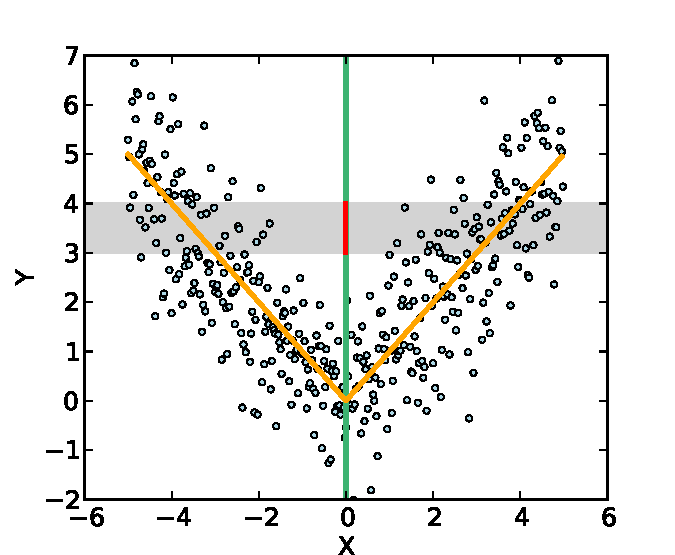
\includegraphics{013.pdf}}
%\end{center}
%
%
%\end{frame}
%
%
%\begin{frame}
%\frametitle{Conditional variance}
%
%For a joint distribution with finite sample spaces, the {\bf
%  conditional variance} is the variance of one of the variables when
%the value of the other variable is held fixed.
%
%This amounts to taking the variance within a row (or within a column)
%of the distribution table.
%
%For example, in the case of this joint distribution (which we saw earlier):
%
%\begin{center}
%\begin{tabular}{llll}
%   & \multicolumn{3}{c}{\rm MTD}\\
%   & 200  & 400  & 600 \\\hline
%A  & 0.6 & 0.3 & 0.1 \\
%B  & 0.1 & 0.5 & 0.4 \\\hline
%\end{tabular}
%\end{center}
%
%The conditional variances given the drug (A or B) are:
%
%\vspace{-0.3cm}
%
%$$
%\begin{array}{ccl}
%{\rm var}({\rm MTD}|{\rm A}) &=& 0.6\cdot(200-300)^2 +
%  0.3\cdot(400-300)^2 + 0.1\cdot(600-300)^2\\ &=& 18,000 \\ {\rm
%  var}({\rm MTD}|{\rm B}) &=& 0.1\cdot(200-460)^2 +
%  0.5\cdot(400-460)^2 + 0.4\cdot(600-460)^2\\ &=& 16,400
%\end{array}
%$$
%
%\vspace{-0.3cm}
%
%Here we are using the conditional means $E({\rm MTD}|{\rm A}) = 300$
%and $E({\rm MTD}|{\rm B}) = 460$.
%
%\end{frame}
%
%
%\begin{frame}
%\frametitle{Conditional variance}
%
%The value of ${\rm var}({\rm MTD}|D=d)$ tells us the variance in MTD
%values among those people who were treated with drug $d$.
%
%In the example above, we see that the subjects treated with drug $A$
%had slightly more variable MTD values than the subjects treated with
%drug $B$.
%
%\end{frame}
%
%
%\begin{frame}
%\frametitle{Law of total variation}
%
%The {\bf law of total variation} relates the marginal variance to the
%conditional means and variances:
%
%$$
%{\rm var}(Y) = {\rm var}_XE(Y|X) + E_X {\rm var}(Y|X).
%$$
%
%Essentially this says that if we are interested in an outcome $Y$, and
%we partition the population into subgroups according to the value of
%another variable $X$, then the variance of $Y$ is the sum of two
%terms:
%
%\begin{itemize}
%
%\item The variance among the mean values of $Y$ in the subgroups
%  defined by different fixed values of $X$.
%
%\item The variance of $Y$ within each subgroup defined by a fixed
%  value of $X$ (averaged over the subgroups).
%
%\end{itemize}
%
%\end{frame}
%
%
%\begin{frame}
%\frametitle{Law of total variation}
%
%\textcolor{blue}{\bf Example:}
%
%\begin{center}
%\scalebox{0.5}{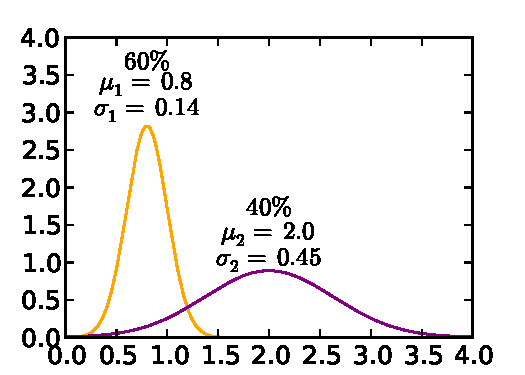
\includegraphics{037.pdf}}
%\end{center}
%
%group = 1,2 are the orange and purple subpopulations
%
%$$ E{\rm var}(Y|{\rm group}) = 0.6\cdot 0.14^2 + 0.4\cdot 0.45^2
%\approx 0.09
%$$
%
%\vspace{-0.7cm}
%
%$$
%EY = E\left( E(Y|{\rm group})\right) = 0.6\cdot 0.8 + 0.4\cdot 2 = 1.28
%$$
%
%\vspace{-0.7cm}
%
%$$
%{\rm var}E(Y|{\rm group}) = 0.6\cdot(0.8-1.28)^2 + 0.4\cdot(2-1.28)^2 = 0.35.
%$$
%
%\vspace{-0.7cm}
%
%$$
%{\rm var}(Y) = 0.09 + 0.35 = 0.44
%$$
%
%\end{frame}
%
%
%\begin{frame}
%\frametitle{Law of total variation}
%
%\textcolor{blue}{\bf Example:} 
%
%Suppose we are comparing two approaches to teaching reading to young
%children, denoted $A$ and $B$.  Each child can be considered to be
%either ``high-risk'' or ``low-risk'' in terms of standard risk factors
%like low family income.  
%
%At the end of the study, reading performance is assessed with a test.
%The risk groups have the following statistical properties:
%
%\begin{itemize}
%
%\item The high-risk subgroup consists of 30\% of the population, and
%  these students have a mean test score of 340, with a standard
%  deviation of 110.
%
%\item The low-risk subgroup consists of 70\% of the population, and
%  these students have a mean test score of 390, with a standard
%  deviation of 70.
%
%\end{itemize}
%
%We can use the law of total variation to determine the overall
%variability of reading test scores.
%
%\end{frame}
%
%\begin{frame}
%\frametitle{Law of total variation}
%
%Let $R=L,H$ denote the risk groups.
%
%First, we compute ${\rm var} E(Y|R)$.  We need the overall mean $EY$:
%
%$$
%EY = E_R E(Y|R) = 0.3\cdot 340 + 0.7\cdot 390 = 375.
%$$
%
%Thus
%
%$$
%{\rm var} E(Y|R) = 0.3\cdot(340-375)^2 + 0.7\cdot(390-375)^2 = 525.
%$$
%
%Next, we compute $E {\rm var}(Y|R)$ as
%
%$$
%0.3\cdot 110^2 + 0.7\cdot 70^2 = 7060.
%$$
%
%We conclude that ${\rm var}(Y) = 525 + 7060 = 7585$, and that
%$525/7585 \times 100\% = 6.9\%$ of the variation in test scores is
%explained by risk group status.
%
%\end{frame}
%
%
%
%\begin{frame}
%\frametitle{Conditional variance for continuous variables}
%
%If $Y|X$ has a normal distribution, around 95\% of the $Y$ values with
%a fixed value $X=x$ will fall in the interval 
%
%$$E(Y|X=x) \pm 2{\rm SD}(Y|X=x),$$ 
%
%where ${\rm SD}(Y|X) = \sqrt{{\rm var}(Y|X)}$.
%
%In the following example, $E(Y|X)$ is the orange line, and ${\rm
%SD}(Y|X) \equiv 1$ is constant.
%
%\begin{center}
%\scalebox{0.5}{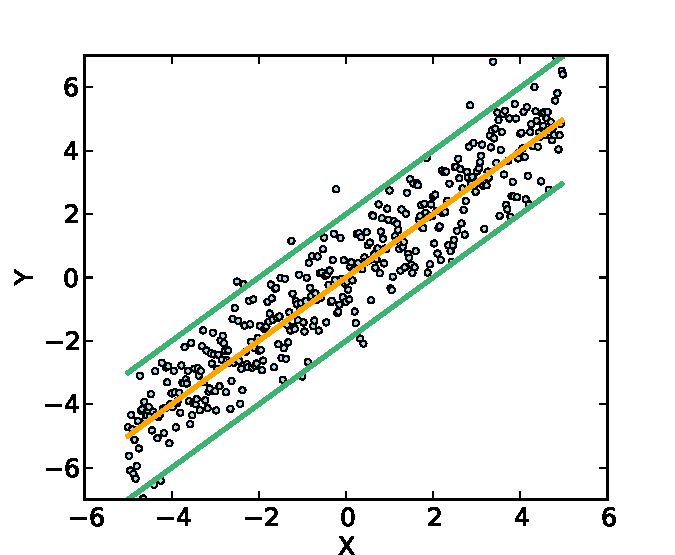
\includegraphics{014_0.pdf}}
%\end{center}
%
%\end{frame}
%
%
%\begin{frame}
%\frametitle{Conditional variance for continuous variables}
%
%In this example, $E(Y|X)$ is the same as above, but now ${\rm
%SD}(Y|X)$ is an increasing function of $X$:
%
%\begin{center}
%\scalebox{0.6}{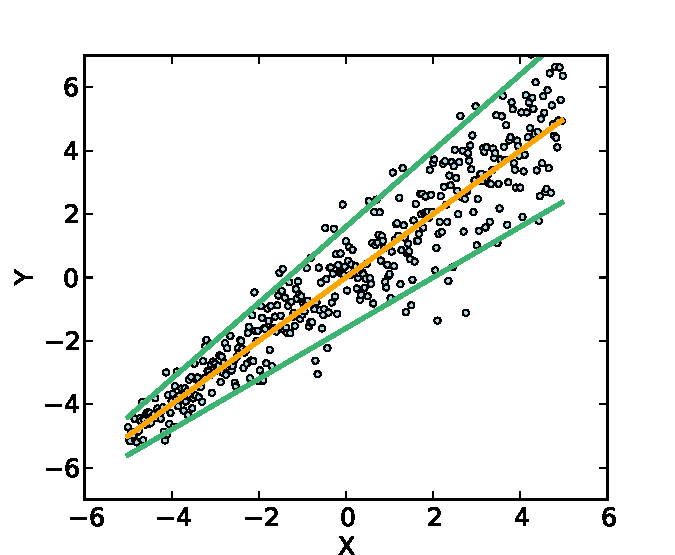
\includegraphics{014_1.pdf}}
%\end{center}
%
%\end{frame}
%
%
%\begin{frame}
%\frametitle{Conditional variance for continuous variables}
%
%In this example $E(Y|X)$ is constant and ${\rm SD}(Y|X)$ is a
%decreasing function of $X$:
%
%\begin{center}
%\scalebox{0.6}{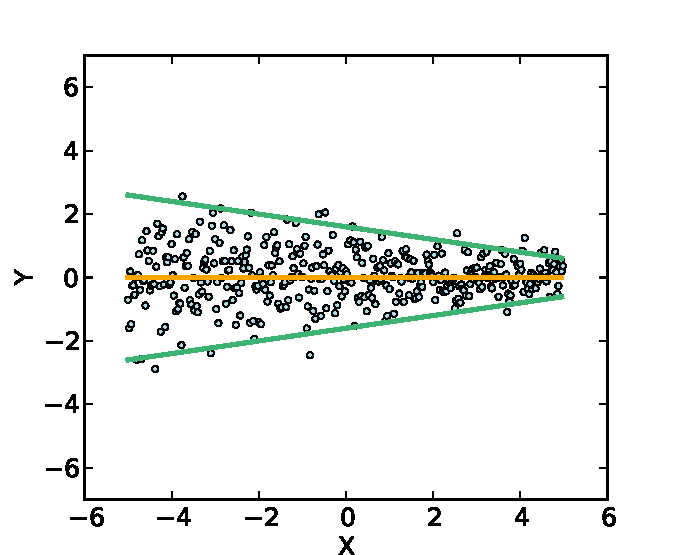
\includegraphics{014_2.pdf}}
%\end{center}
%
%\end{frame}
%
%
%\begin{frame}
%\frametitle{Law of total variation for continuous variables}
%
%Recall that the low of total variation states that ${\rm var}(Y) = {\rm
%var}E(Y|X) + E{\rm var}(Y|X)$.
%
%In this example, $E(Y|X) \equiv 0$ so ${\rm var}E(Y|X) = 0$, and ${\rm
%var}(Y|X) = 1$ so $E{\rm var}(Y|X) \equiv 1$.  Thus ${\rm var}(Y) =
%1$.
%
%\begin{center}
%\scalebox{0.6}{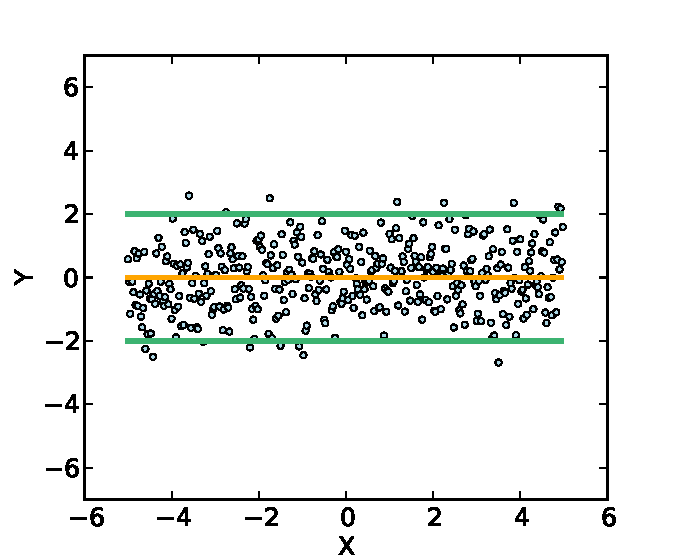
\includegraphics{014_3.pdf}}
%\end{center}
%
%\end{frame}
%
%
%\begin{frame}
%\frametitle{Law of total variation for continuous variables}
%
%In this example ${\rm var}E(Y|X) = 0$ as above, but ${\rm var}(Y|X)$
%ranges from 1.7 (when $X=-5$) to 0.1 (when $X=5$).  If we average
%${\rm var}(Y|X)$ over the $X$ distribution we get $E{\rm var}(Y|X) =
%0.73$, which is also the variance of $Y$.
%
%\begin{center}
%\scalebox{0.6}{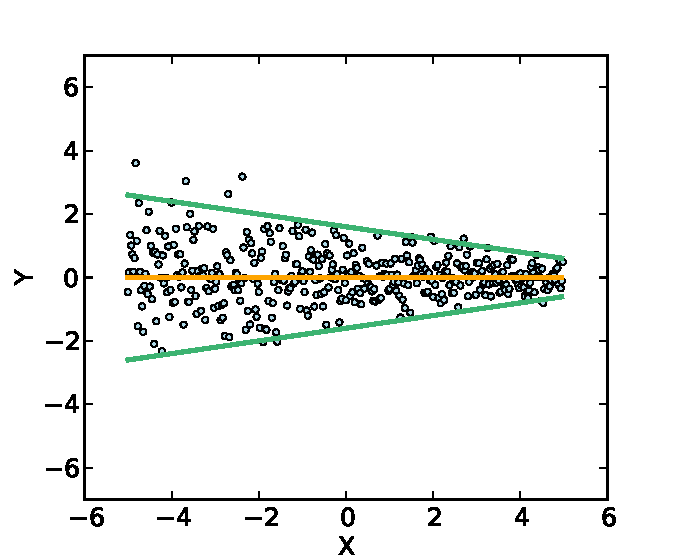
\includegraphics{014_4.pdf}}
%\end{center}
%
%\end{frame}
%
%
%\begin{frame}
%\frametitle{Law of total variation for continuous variables}
%
%In this example $E(Y|X)$ ranges from -5 (when $X=-5$) to 5 (when
%$X=5$).  If we take the variance of these values over the $X$
%distribution, we get ${\rm var} E(Y|X) = 8.3$.  ${\rm var}(Y|X)$ is
%constant at $1$ for all $X$ values, so its mean value is also $1$.
%Thus the variance of $Y$ is $8.3 + 1 = 9.3$.
%
%\begin{center}
%\scalebox{0.6}{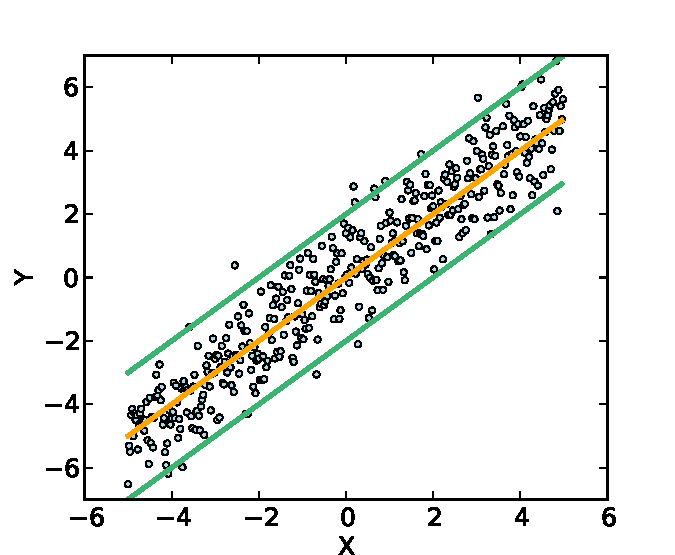
\includegraphics{014_5.pdf}}
%\end{center}
%
%\end{frame}
%
%
%\begin{frame}
%\frametitle{Law of total variation for continuous variables}
%
%In this example ${\rm var}E(Y|X) = 8.3$ as above, and ${\rm var}(Y|X)$
%ranges from 0.09 (when $X=-5$) to 1.68 (when $X=5$).  It turns out
%that $E{\rm var}(Y|X) = 0.72$.  Thus the variance of $Y$ is $8.3 +
%0.72 = 9.02$.
%
%\begin{center}
%\scalebox{0.6}{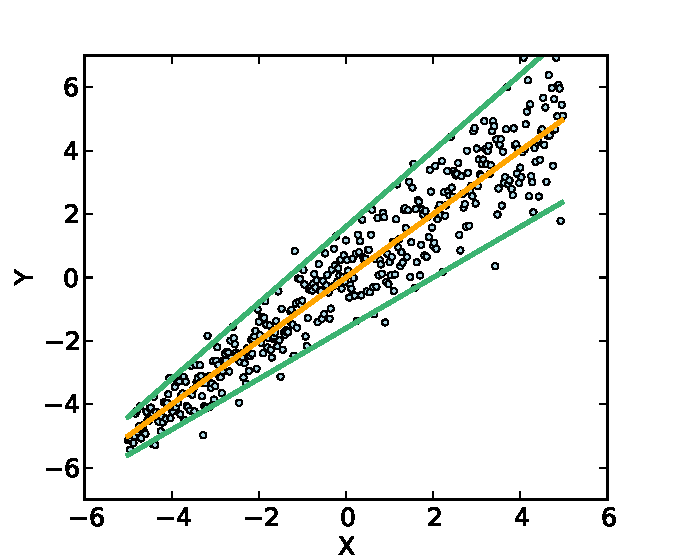
\includegraphics{014_6.pdf}}
%\end{center}
%
%\end{frame}
